% figure: 现控1-21-模拟变量图.png
% Six-state analog diagram, with arbitrary integrator initial conditions.
% x1'=x2, x2'=x3, x3'=-6*x1-11*x2-6*x3+u.
% x4'=-5*x4, x5'=-7*x5+x6, x6'=-7*x6+4*u, y=x1+x4.
\documentclass[border=10pt]{standalone}
\usepackage{fontspec}
\setmainfont{Cambria}
\usepackage{unicode-math}
\setmathfont{Cambria Math}
\usepackage{tikz}
\usetikzlibrary{arrows.meta,calc}

\definecolor{ink}{HTML}{1E2228}
\definecolor{fillblue}{HTML}{E8EFF8}
\definecolor{muted}{HTML}{606874}

\begin{document}
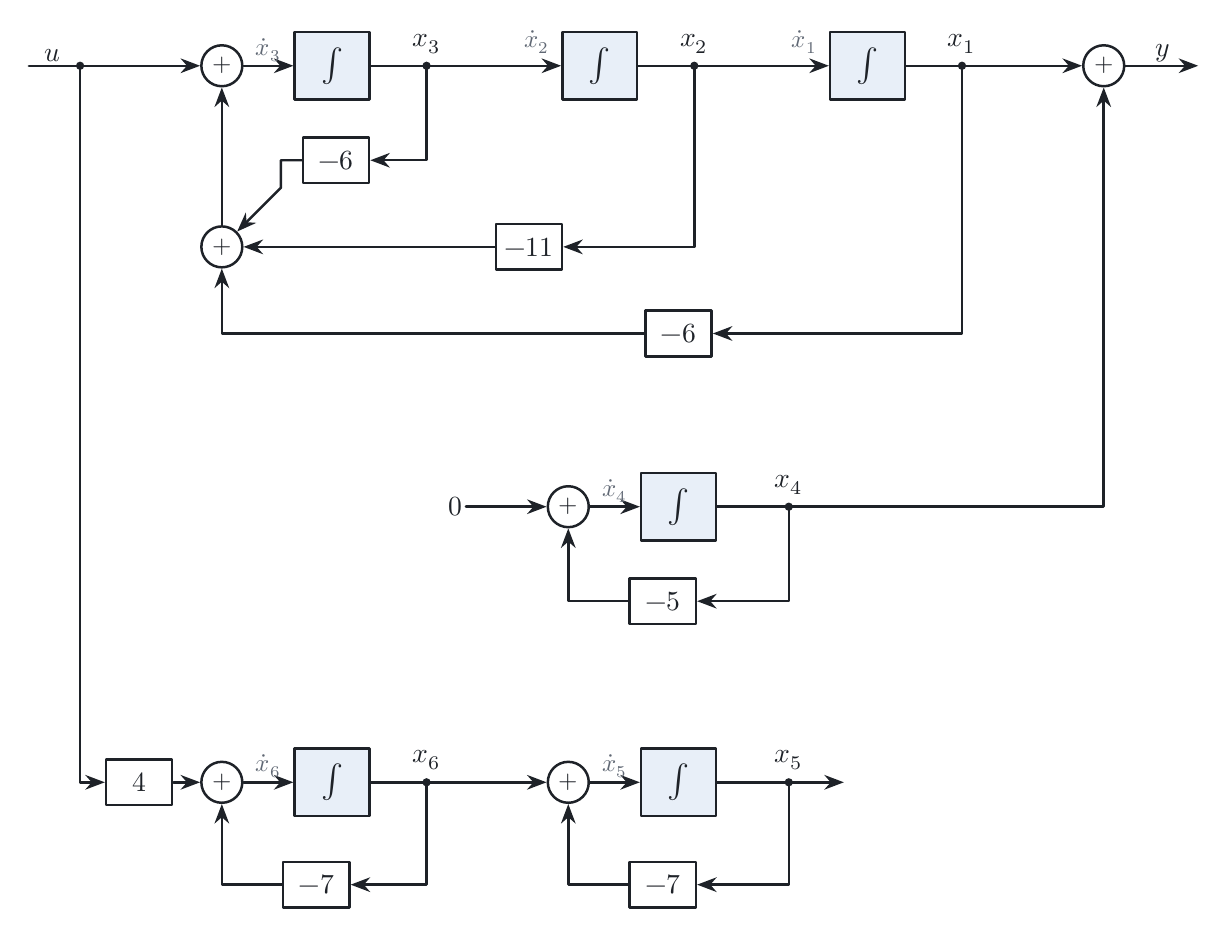
\begin{tikzpicture}[
  x=1cm,y=1cm,draw=ink,text=ink,
  line width=0.9pt,line cap=round,line join=round,
  >=Stealth,
  sum/.style={draw,circle,minimum size=0.52cm,inner sep=0pt,font=\small},
  intg/.style={draw,fill=fillblue,minimum width=0.95cm,
    minimum height=0.86cm,inner sep=1pt,font=\large},
  gain/.style={draw,fill=white,minimum width=0.84cm,
    minimum height=0.58cm,inner sep=2pt,font=\normalsize},
  sig/.style={font=\normalsize,inner sep=1pt},
  deriv/.style={font=\small,text=muted,inner sep=1pt}
]

% Main controllable chain, drawn in integration order x3 -> x2 -> x1.
\node[sum] (s3) at (1.8,7.4) {$+$};
\node[intg] (i3) at (3.2,7.4) {$\int$};
\node[intg] (i2) at (6.6,7.4) {$\int$};
\node[intg] (i1) at (10.0,7.4) {$\int$};
\coordinate (x3) at (4.4,7.4);
\coordinate (x2) at (7.8,7.4);
\coordinate (x1) at (11.2,7.4);
\node[sum] (sy) at (13.0,7.4) {$+$};

\draw[->] (-0.65,7.4) -- node[sig,above,pos=0.14] {$u$} (s3.west);
\draw[->] (s3.east) -- node[deriv,above] {$\dot x_3$} (i3.west);
\draw[->] (i3.east) -- (i2.west);
\draw[->] (i2.east) -- (i1.west);
\draw[->] (i1.east) -- (sy.west);
\node[sig,above=3pt] at (x3) {$x_3$};
\node[sig,above=3pt] at (x2) {$x_2$};
\node[sig,above=3pt] at (x1) {$x_1$};
\node[deriv,above=3pt] at (5.8,7.4) {$\dot x_2$};
\node[deriv,above=3pt] at (9.2,7.4) {$\dot x_1$};
\draw[->] (sy.east) -- node[sig,above] {$y$} (14.2,7.4);

% Signed feedback gains meet at an explicit adder, never a wire junction.
\node[sum] (sf) at (1.8,5.1) {$+$};
\node[gain] (g3) at (3.25,6.2) {$-6$};
\node[gain] (g2) at (5.7,5.1) {$-11$};
\node[gain] (g1) at (7.6,4.0) {$-6$};
\draw[->] (x3) -- (4.4,6.2) -- (g3.east);
\draw[->] (g3.west) -- (2.55,6.2) -- (2.55,5.85) -- (sf.north east);
\draw[->] (x2) -- (7.8,5.1) -- (g2.east);
\draw[->] (g2.west) -- (sf.east);
\draw[->] (x1) -- (11.2,4.0) -- (g1.east);
\draw[->] (g1.west) -- (1.8,4.0) -- (sf.south);
\draw[->] (sf.north) -- (s3.south);

% Autonomous x4: its nonzero initial state can still affect the output.
\node[sum] (s4) at (6.2,1.8) {$+$};
\node[intg] (i4) at (7.6,1.8) {$\int$};
\node[gain] (g4) at (7.4,0.6) {$-5$};
\coordinate (x4) at (9.0,1.8);
\draw[->] (4.9,1.8) node[sig,left] {$0$} -- (s4.west);
\draw[->] (s4.east) -- node[deriv,above] {$\dot x_4$} (i4.west);
\draw[->] (i4.east) -- (13.0,1.8) -- (sy.south);
\node[sig,above=3pt] at (x4) {$x_4$};
\draw[->] (x4) -- (9.0,0.6) -- (g4.east);
\draw[->] (g4.west) -- (6.2,0.6) -- (s4.south);

% Jordan chain: 4*u drives x6, then x6 drives x5. Neither enters y.
\node[gain] (b6) at (0.75,-1.7) {$4$};
\node[sum] (s6) at (1.8,-1.7) {$+$};
\node[intg] (i6) at (3.2,-1.7) {$\int$};
\node[sum] (s5) at (6.2,-1.7) {$+$};
\node[intg] (i5) at (7.6,-1.7) {$\int$};
\coordinate (x6) at (4.4,-1.7);
\coordinate (x5) at (9.0,-1.7);
\node[gain] (g6) at (3.0,-3.0) {$-7$};
\node[gain] (g5) at (7.4,-3.0) {$-7$};
\draw[->] (0,7.4) -- (0,-1.7) -- (b6.west);
\draw[->] (b6.east) -- (s6.west);
\draw[->] (s6.east) -- node[deriv,above] {$\dot x_6$} (i6.west);
\draw[->] (i6.east) -- (s5.west);
\node[sig,above=3pt] at (x6) {$x_6$};
\draw[->] (s5.east) -- node[deriv,above] {$\dot x_5$} (i5.west);
\draw[->] (i5.east) -- (9.7,-1.7);
\node[sig,above=3pt] at (x5) {$x_5$};
\draw[->] (x6) -- (4.4,-3.0) -- (g6.east);
\draw[->] (g6.west) -- (1.8,-3.0) -- (s6.south);
\draw[->] (x5) -- (9.0,-3.0) -- (g5.east);
\draw[->] (g5.west) -- (6.2,-3.0) -- (s5.south);

% Dots occur only at actual signal fan-outs.
\foreach \p in {x1,x2,x3,x4,x5,x6}
  \fill[ink] (\p) circle (1.5pt);
\fill[ink] (0,7.4) circle (1.5pt);

\end{tikzpicture}
\end{document}
